\documentclass[11pt]{article}

\usepackage{fullpage}
\usepackage{amsfonts}
\usepackage{graphicx}

\def\eq1{y=\frac{x}{3x^2+x+1}}
\def\labelaxes{Remember to include a scale and label your axes.}

\begin{document}

The set of Natural numbers is denoted by $\mathbb{N}$.

The set of integers is denoted by $\mathbb{Z}$.

The set of real numbers is denoted by $\mathbb{R}$

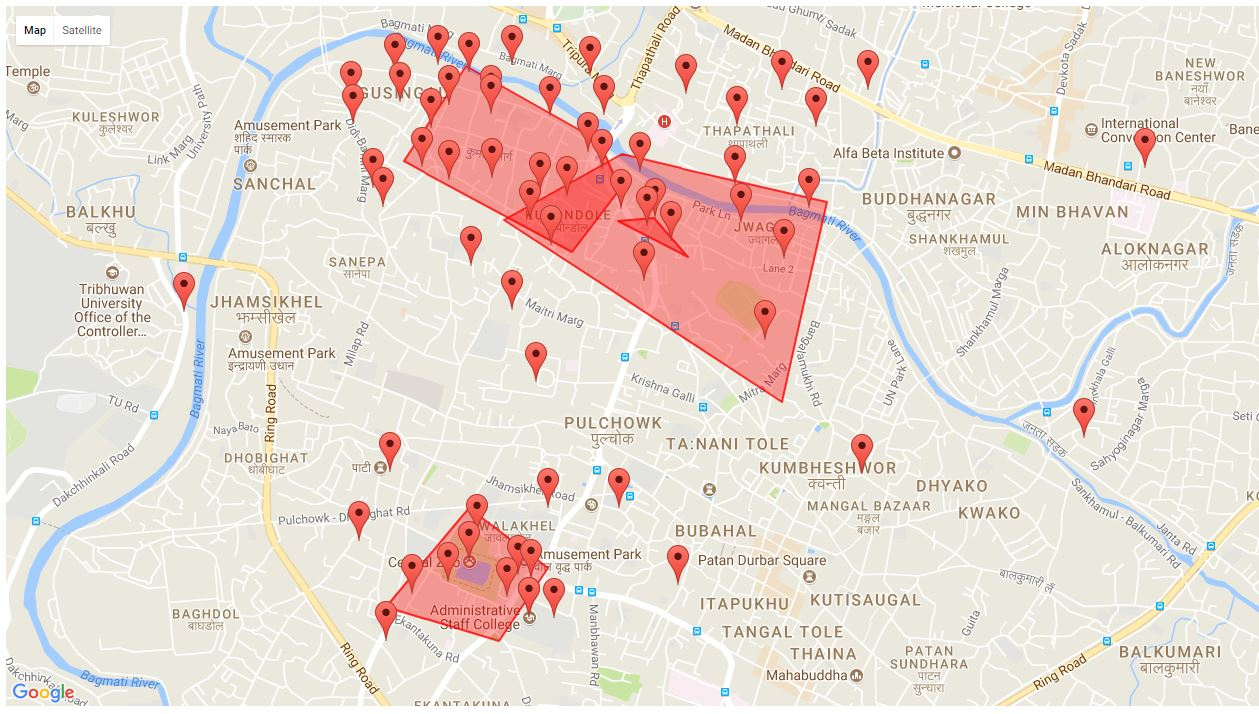
\includegraphics[width=6in]{test_01.jpg}

Graph: $\displaystyle \eq1$\\
\labelaxes

Remember that images must be saved as .png, .jpg, .gif or .pdf files
\begin{center}
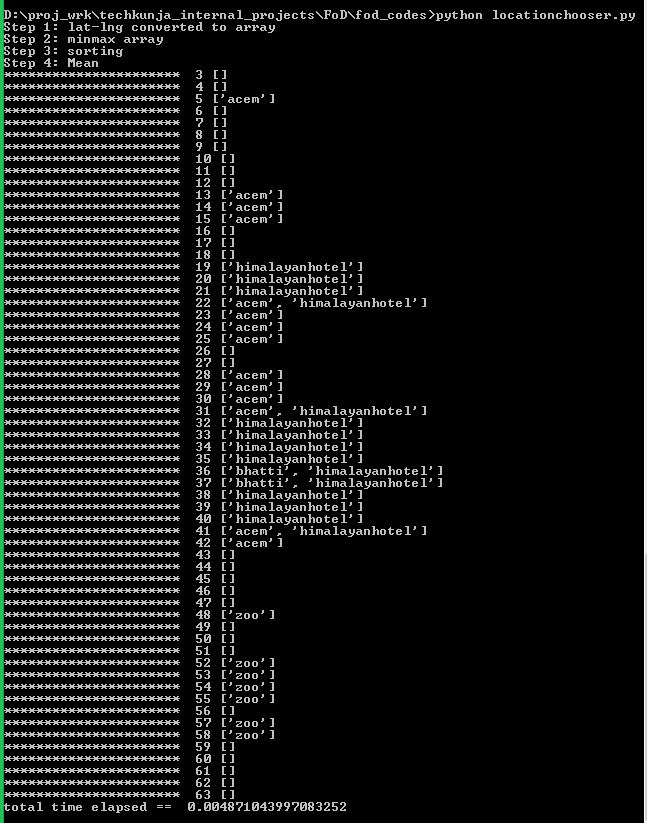
\includegraphics[width=5in, angle=90]{test_02.jpg}
\end{center}


\end{document}